\documentclass[12pt]{article}

%%%%%%%%%%%%%%%%%%%%%%%%%%%%%%%%%%%%%%%%%%%%%%%%%%%%%%%%%%%%%%%%%%%%%%%%%%%%%%%%%%%%%%%%%%%%%%%%%%%%
% Math
\usepackage{fancyhdr} 
\usepackage{amsfonts}
\usepackage{amsmath}
\usepackage{amssymb}
\usepackage{amsthm}
%\usepackage{dsfont}

%%%%%%%%%%%%%%%%%%%%%%%%%%%%%%%%%%%%%%%%%%%%%%%%%%%%%%%%%%%%%%%%%%%%%%%%%%%%%%%%%%%%%%%%%%%%%%%%%%%%
% Macros
\usepackage{calc}

%%%%%%%%%%%%%%%%%%%%%%%%%%%%%%%%%%%%%%%%%%%%%%%%%%%%%%%%%%%%%%%%%%%%%%%%%%%%%%%%%%%%%%%%%%%%%%%%%%%%
% Commands and Custom Variables	
\newcommand{\problem}[1]{\hspace{-4 ex} \large \textbf{Problem #1} }
\let\oldemptyset\emptyset
\let\emptyset\varnothing
\newcommand{\norm}[1]{\left\lVert#1\right\rVert}
\newcommand{\sint}{\text{s}\kern-5pt\int}
\newcommand{\powerset}{\mathcal{P}}
\renewenvironment{proof}{\hspace{-4 ex} \emph{Proof}:}{\qed}
\newcommand{\RR}{\mathbb{R}}
\newcommand{\NN}{\mathbb{N}}
\newcommand{\QQ}{\mathbb{Q}}
\newcommand{\ZZ}{\mathbb{Z}}
\newcommand{\CC}{\mathbb{C}}
\renewcommand{\Re}{\operatorname{Re}}
\renewcommand{\Im}{\operatorname{Im}}


%%%%%%%%%%%%%%%%%%%%%%%%%%%%%%%%%%%%%%%%%%%%%%%%%%%%%%%%%%%%%%%%%%%%%%%%%%%%%%%%%%%%%%%%%%%%%%%%%%%%
%page
\usepackage[margin=1in]{geometry}
\usepackage{setspace}
%\doublespacing
\allowdisplaybreaks
\pagestyle{fancy}
\fancyhf{}
\rhead{Shaw \space \thepage}
\setlength\parindent{0pt}

%%%%%%%%%%%%%%%%%%%%%%%%%%%%%%%%%%%%%%%%%%%%%%%%%%%%%%%%%%%%%%%%%%%%%%%%%%%%%%%%%%%%%%%%%%%%%%%%%%%%
%Code
\usepackage{listings}
\usepackage{courier}
\lstset{
	language=Python,
	showstringspaces=false,
	formfeed=newpage,
	tabsize=4,
	commentstyle=\itshape,
	basicstyle=\ttfamily,
}

%%%%%%%%%%%%%%%%%%%%%%%%%%%%%%%%%%%%%%%%%%%%%%%%%%%%%%%%%%%%%%%%%%%%%%%%%%%%%%%%%%%%%%%%%%%%%%%%%%%%
%Images
\usepackage{graphicx}
\graphicspath{ {images/} }
\usepackage{float}

%tikz
\usepackage[utf8]{inputenc}
\usepackage{pgfplots}
\usepgfplotslibrary{groupplots}

%%%%%%%%%%%%%%%%%%%%%%%%%%%%%%%%%%%%%%%%%%%%%%%%%%%%%%%%%%%%%%%%%%%%%%%%%%%%%%%%%%%%%%%%%%%%%%%%%%%%
%Hyperlinks
%\usepackage{hyperref}
%\hypersetup{
%	colorlinks=true,
%	linkcolor=blue,
%	filecolor=magenta,      
%	urlcolor=cyan,
%}

\begin{document}
	\thispagestyle{empty}
	
	\begin{flushright}
		Sage Shaw \\
		m565 - Fall 2017 \\
		\today
	\end{flushright}
	
{\large \textbf{HW 7}}\bigbreak

%%%%%%%%%%%%%%%%%%%%%%%%%%%%%%%%%%%%%%%%%%%%%%%%%%%%%%%%%%%%%%%%%%%%%%%%%%%%%%%%%%%%%%%%%%%%%%%%%%%%
\problem{1 (a)} The following code computes the error using the Trapezoidal rule applied to the functions
\begin{align*}
	I(f_1) & = \int_{-1}^1 (x-1)^2e^{-x^2}dx \\
	I(f_2) & = \int_{-1}^1 e^{\cos(\pi x)} dx
\end{align*}

\begin{lstlisting}
def trap_int(f, a, b, n):
	h = (b-a)/n
	x = a + h
	T = 0
	for i in range(n-1):
	T += f(x)
	x += h
	T += (f(a)+f(b))/2
	T *= h
	return T

def f1(x):
	return (x-1)**2 * np.exp(-x**2)

def f2(x):
	return np.exp( np.cos( np.pi*x ) )

int1_actual = 1.87259295726583875
int2_actual = 2.53213175550401667

def p1a():
	ns = [4, 8, 16, 32]
	T1 = []
	T2 = []
	for n in ns:
		T1.append( abs( trap_int(f1, -1, 1, n) - int1_actual ) )
		T2.append( abs( trap_int(f2, -1, 1, n) - int2_actual ) )
	latex_table( (ns, T1, T2), 
('$n$', '$I(f_1)$ error', '$I(f_2)$ error') )
\end{lstlisting}

	The output is displayed in the table below.
	\begin{center}
		\begin{tabular}{|c|c|c|}
			\hline
			$n$&$I(f_1)$ error&$I(f_2)$ error\\ \hline
			4&0.0312125372551&0.0109488793112\\ \hline
			8&0.0076967258198&3.98424961467e-07\\ \hline
			16&0.001918044355&4.4408920985e-16\\ \hline
			32&0.000479134582236&4.4408920985e-16\\ \hline
		\end{tabular}
	\end{center}

\bigbreak
%%%%%%%%%%%%%%%%%%%%%%%%%%%%%%%%%%%%%%%%%%%%%%%%%%%%%%%%%%%%%%%%%%%%%%%%%%%%%%%%%%%%%%%%%%%%%%%%%%%%
\problem{1 (b)} The following code does the same for the corrected Trapezoidal rule:

	\begin{lstlisting}
def df1(x):
	return 2*(x-1)*np.exp(-x**2) - 2*x*(x-1)**2 * np.exp(-x**2)

def df2(x):
	return -np.pi*np.sin(np.pi*x)*np.exp(np.cos(np.pi*x))

def trap_int_corrected(f, df, a, b, n):
	T = trap_int(f,a,b,n)
	h = (b-a)/n 
	return T - h**2/12*(df(b)-df(a))

def p1b():
	int1_actual = 1.87259295726583875
	int2_actual = 2.53213175550401667
	ns = [4, 8, 16, 32]
	T1 = []
	T2 = []
	for n in ns:
		T1.append( abs( trap_int_corrected(f1, df1, -1, 1, n)
- int1_actual ) )
		T2.append( abs( trap_int_corrected(f2, df2, -1, 1, n)
- int2_actual ) )
	latex_table( (ns, T1, T2), 
('$n$', '$I(f_1)$ error', '$I(f_2)$ error') ) 
	\end{lstlisting}
	
	\begin{center}
		\begin{tabular}{|c|c|c|}
			\hline
			$n$&$I(f_1)$ error&$I(f_2)$ error\\ \hline
			4&0.00055591715752&0.0109488793112\\ \hline
			8&3.25707953921e-05&3.98424961467e-07\\ \hline
			16&2.00559889851e-06&4.4408920985e-16\\ \hline
			32&1.24893210662e-07&4.4408920985e-16\\ \hline
		\end{tabular}
	\end{center}


\bigbreak
%%%%%%%%%%%%%%%%%%%%%%%%%%%%%%%%%%%%%%%%%%%%%%%%%%%%%%%%%%%%%%%%%%%%%%%%%%%%%%%%%%%%%%%%%%%%%%%%%%%%
\problem{1 (c)} To verify that the error of the Trapezoidal rule decreases like $\mathcal{O}(h^2)$ We plot $h^2$ with the error. (More data points have been calcluated for this plot.)
	\begin{figure}[H]
		\caption{Error of the trapezoidal rule}
		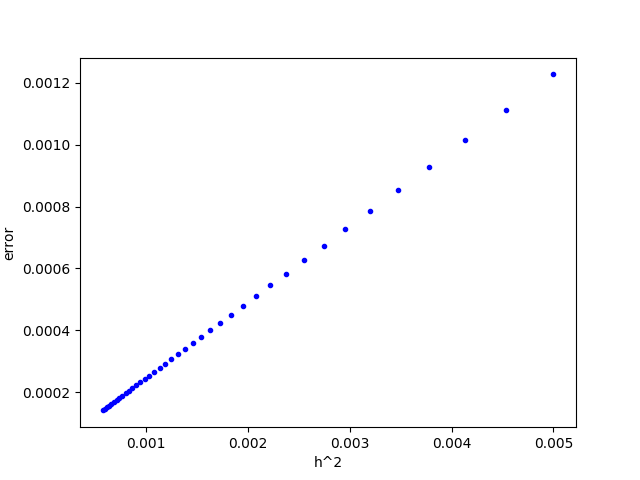
\includegraphics[width=.75\textwidth]{hw7_p1_fig1}
		\label{p1_T_err}
		\centering
	\end{figure}
	Since the plot is roughly linear we can confirm that the error decreases like $\mathcal{O}(h^2)$. \bigbreak

	Similarly a plot of $h^4$ with the error of the corrected Trapezoidal rule shows that its error decreaces according to $\mathcal{O}(h^4)$.
	\begin{figure}[H]
		\caption{Error of the corrected trapezoidal rule}
		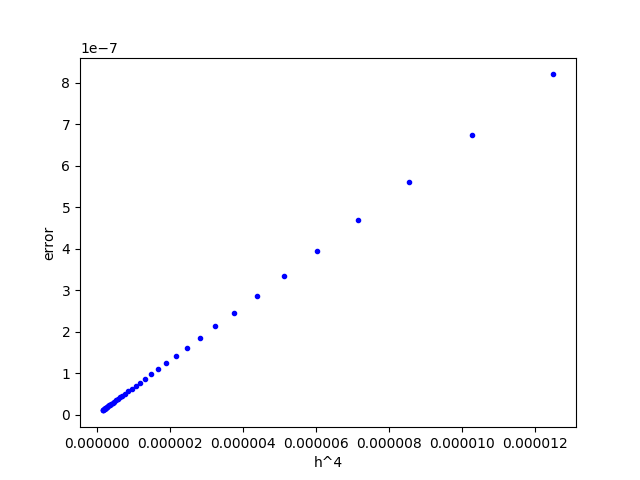
\includegraphics[width=.75\textwidth]{hw7_p1_fig2}
		\label{p1_T_corrected_err}
		\centering
	\end{figure}

\bigbreak
%%%%%%%%%%%%%%%%%%%%%%%%%%%%%%%%%%%%%%%%%%%%%%%%%%%%%%%%%%%%%%%%%%%%%%%%%%%%%%%%%%%%%%%%%%%%%%%%%%%%
\problem{1 (d)} The rate of the error of the Trapezoidal rule applied to $I(f_2)$ will acually decreace along $\mathcal{O}(h^4)$. This is because $f_2^\prime(-1)=0= f_2^\prime(1)$ and thus the correction term for the corrected Trapezoidal rule is $0$. For the same justification that the error of the corrected trapezoidal rule decreaces by $\mathcal{O}(h^4)$ we can justify that the uncorrected Trapazoidal rule will too, since it has the same value.

\bigbreak
%%%%%%%%%%%%%%%%%%%%%%%%%%%%%%%%%%%%%%%%%%%%%%%%%%%%%%%%%%%%%%%%%%%%%%%%%%%%%%%%%%%%%%%%%%%%%%%%%%%%
\problem{2 (a)}


\end{document}
